\documentclass{article}
\usepackage[utf8]{inputenc}

\title{}


\title{%
  Text Mining for Information Retrieval on WikIR \\
  \large Project for Machine Learning course}
\author{Jakub Bartczuk}
\date{Winter 2020}

\usepackage{natbib}
\usepackage{graphicx}
\usepackage{url}
\usepackage{hyperref}
\usepackage{csvsimple}
\usepackage{multirow}

\begin{document}

\maketitle

\section{Motivation}
One of the first things that data scientists do when facing a new problem is searching for related problems and software on GitHub. GitHub's search capabilities are very limited (at the time of writing this report) - there are several features like project descriptions, tags and readmes that could be helpful, but its search engine doesn't allow for searching them simultaneously. The effect is that sometimes reformulating query might result in drastically different search results. This project aims at evaluating in a controlled experiment several simple text mining methods that can be useful for expanding traditional bag-of-words retrieval model.

\section{Abstract}

WikIR \citep{frej2019wikir} is a recently proposed dataset for evaluating Information Retrieval. So far it was used only to benchmark standard Information Retrieval method (BM25)\citep{manning2008introduction} versus deep learning-based text matching. In this project several machine learning methods for text, using classification, word embeddings and matrix decomposition were used to improve searching results.

\section{Dataset}
The dataset consists of approx. 100k documents and queries split into training, validation and test sets (with 1k, 100 and 100 examples respectively). It is created from wikipedia articles and their titles: queries are the titles, whereas rest of article (with first paragraph removed) gets split into 'documents' to be retrieved. Document is deemed relevant for query if either the query is the title of document's article (relevance score 2) or its article is linked in retrieved document's article. Below query lengths are reported. Document lengths are less interesting, since author's method splits articles into documents of approx. 200 words.

\begin{figure}[h!]
\centering
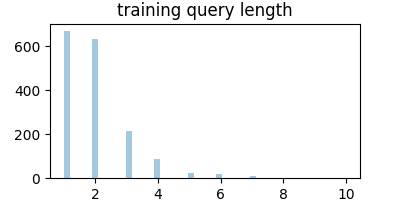
\includegraphics[scale=0.7]{images/training_query_length.png}
\label{fig:universe}
\end{figure}

\begin{figure}[h!]
\centering
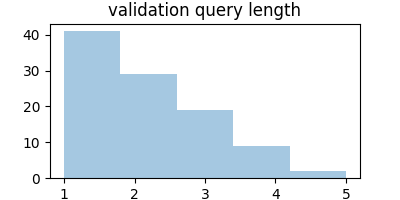
\includegraphics[scale=0.7]{images/validation_query_length.png}
\label{fig:universe}
\end{figure}

\begin{figure}[h!]
\centering
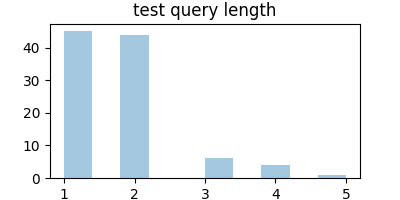
\includegraphics[scale=0.7]{images/test_query_length.png}
\label{fig:universe}
\caption{Query lengths (in words) histograms}
\end{figure}

\section{Evaluation}

All methods apart from query expansion-based retriever first retrieve 100 records using BM25 relevance model and then perform reranking.

Results are evaluated using standard Information Retrieval metrics: Precision at $k$, nDCG at $k$ and Mean Average Precision.

\section{Data preparation} 
For our models we preprocess data according to original paper: english stop words are removed and the words are stemmed using Porter stemmer. These steps are performed using NLTK \citep{Loper02nltk:the}.

Models were tested with both stemmed and unstemmed texts. Also, keyword extraction was used as a step for some word embedding models (to alleviate problem of averaging larege documents). Keyword extraction was performed using gensim's \citep{rehurek_lrec} textrank model.

\section{Models}

\begin{enumerate}

  \item Baseline - relevance ranking using Okapi BM25 \citep{bm25_impro} model.
  \item Classification on BM25 features and tf-idf features \citep{DBLP:journals/corr/abs-1904-08861}
  
  Bag of words features are used for classification with logistic regression. It is trained on first $k$ (positive) and last $k$ (negative) documents retrieved using BM25. Classifier probability scores $p_i$ and BM25 relevance $r_i$ are then weighted and documents are ranked using $r_i' = \alpha p_i + (1 - \alpha) r_i$
  \item Classification on using GloVe \citep{Pennington14glove:global} and FastText \citep{bojanowski2016enriching}  word embeddings
  
  Classification is performed as in step 1, but using word embedding features. These are averaged embeddings for words from used column.
  
  \item Scoring using similarity based on unsupervised representation (using Nonnegative Matrix Factorization)
  
  NMF is trained on whole documents corpus, and new relevance is defined as $r_i' = \alpha s_i + (1 - \alpha) r_i$ Where $s_i = S(v_{q_i}, v_{d_i})$ Where $v_{t}$ is NMF features for text $t$, and $S$ denotes cosine similarity.
  
  \item Query expansion using nearest neighbor word embeddings.
  
Models 1-3 work by combining their score with relevance score. BM25 model is first used to retrieve 100 top documents. Model score results from running classification: top $k$ are defined as positive and bottom $k$ documents are defined as negative.
  
\end{enumerate}

\section{Results}


\begin{tabular}{l*{8}{c}}
& method & MAP & P@5 & P@10 & P@20 & NDCG@5 & NDCG@10 & NDCG@20 \\
\hline
1. & baseline & 0.1985 & 0.322 & 0.238 & \textbf{0.172} & 0.4249 & 0.3861 & 0.39477\\
2. & classifier retriever & 0.1989 & 0.328 & 0.24 & 0.17 & \textbf{0.4308} & 0.3888 & \textbf{0.395} \\
3. & word embedding retriever & \textbf{0.2064} & \textbf{0.33} & \textbf{0.242} & 0.166 & 0.433 & \textbf{0.3946} & 0.394\\
4. & unsupervised retriever & 0.1782 & 0.29 & 0.206 & 0.1555 & 0.3905 & 0.3487 & 0.3612\\
5. & query expander & 0.0968 & 0.14 & 0.126 & 0.096 & 0.1951 & 0.1971 & 0.2138\\

\hline
\end{tabular}

\subsection{Best hyperparameters}
Following hyperparameters were used (1 and 5 do not have hyperparameters). Text denotes whether method used text, 10 keywords extracted with TextRank or stemmed text. n\_used\_documents means that top $n$ and bottom $n$ documents were used for classification. 

2. Uses $\alpha = 0.3$, text = keywords,  n\_used\_documents=20 \\

3. $\alpha = 0.4$, text = keywords \\ 

4. $\alpha = 0.1$, text = stemmed text, n\_components = 100 \\


\section{Deliverables}

Project's code can be found on its GitHub page\footnote{\href{https://github.com/lambdaofgod/wikir_text_mining}{https://github.com/lambdaofgod/wikir\_text\_mining}}. For experiment management guild.ai\footnote{\href{https://github.com/guildai/guildai}{https://github.com/guildai/guildai}} tool was used. Project provides \texttt{Retriever} class that wraps ranking models giving different methods common interface.

\section{Conclusion}
BM25 already provides strong baseline for search results ranking. The difference noted in Lin's paper \citep{DBLP:journals/corr/abs-1904-08861} (linear classifier on bag-of-words features beating BM25 by 2\% MAP) does not happen for WikIR, most likely because of the fact that WikIR queries are very short. It remains an open question whether the results can be improved by using simple machine learning models on top of features extracted using deep learning models.

\section{Further steps}
\begin{itemize}
    \item \textbf{use Learning to Rank approach} - this is intuitively next step after approach that uses classifiers. For example several gradient boosting libraries support ranking models.
    \item \textbf{use word embedding features for global search} - there are methods for building large scale approximate kNNs. These might alleviate query vocabulary mismatch problem.
    \item \textbf{use language-model based features} - recent neural network models in NLP, like Transformers or UMLFiT can be used for extracting document features. These work better than averaging word embeddings.
    \item \textbf{use dataset construction method on another source}
\end{itemize}

\bibliographystyle{plain}
\bibliography{references}
\end{document}